\chapter{File System(FS)}
\label{ch:FS}
\section{Files}
It is essential that a computer system has a facility for storing data over longer periods of time
and for retrieving the stored data. Such a facility is called a FS. Evidently, a FS
cannot accommodate all possible data types and structures that will be programmed in the future.
Hence, it is necessary to provide a simple, yet flexible enough base structure that allows any data
structure to be mapped onto this base structure (and vice-versa) in a reasonably straight-forward
and efficient way. This base structure, called file, is a sequence of bytes. As a consequence, any
given structure to be transformed into a file must be sequentialized. The notion of sequence is
indeed fundamental, and it requires no further explanation and theory. We recall that texts are
sequences of characters, and that characters are typically represented as bytes.

The sequence is also the natural abstraction of all physically moving storage media. Among them
are magnetic tapes and disks. Magnetic media have the welcome property of non-volatility and
are therefore the primary choices for storing data over longer periods of time, especially over
periods where the equipment is switched off. Sequential access is also necessary for media that
allow access only by large blocks, such as flash-RAMs and SD-cards.

A further advantage of the sequence is that its transmission between media is simple too. The
reason is that its structural information is inherent and need not be encoded and transmitted in
addition to the actual data. This implicitness of structural information is particularly convenient in
the case of moving storage media, because they impose strict timing constraints on transmission
of consecutive elements. Therefore, the process which generates (or consumes) the data must
be effectively decoupled from the transmission process that observes the timing constraints. In
the case of sequences, this decoupling is simple to achieve by dividing a sequence into
subsequences which are buffered. A sequence is output to the storage medium by alternately
generating data (and filling the buffer holding the current subsequence) and transmitting data
(fetching elements from the buffer and transmitting them). The size of the subsequences (and the
buffer) depends on the storage medium under consideration: there must be no timing constraints
between accesses to consecutive subsequences.

The file is not a static data structure like the array or the record, because the length may increase
dynamically, i.e. during program execution. On the other hand, the sequence is less flexible than
general dynamic structures, because it cannot change its form, but only its length, since elements
can only be appended but not inserted. It might therefore be called a semi-dynamic structure.
The discipline of purely sequential access to a file is enforced by restricting access to calls of
specific procedures, typically read and write procedures for scanning and generating a file. In the
jargon of data processing, a file must be opened before reading or writing is possible. The
opening implies the initialization of a reading and writing mechanism, and in particular the fixing of
its initial position. Hence each (opened) file not only has a value and a length, but also a position
attributed to it. If reading must occur from several positions (still sequentially) alternately, the file
is "multiply opened"; it implies that the same file is represented by several variables, each
denoting a different position.

This widespread view of files is conceptually unappealing, and the Oberon FS therefore
departs from it by introducing the notion of a rider. A file simply has a value, the sequence of
bytes, and a length, the number of bytes in the sequence. Reading and writing occurs through a
rider, which denotes a position. "Multiple opening" is achieved by simply using several riders
riding on the same file. Thereby the two concepts of data structure (file) and access mechanism
(rider) are clearly distinct and properly disentangled.

Given a file f, a rider r is placed on a file by the call Files.Set (r, f, pos), where pos indicates the
position from which reading or writing is to start. Calls of Files.Read (r, x) and Files.Write (r, x)
implicitly increment the position beyond the element read or written, and the file is implicitly
denoted via the explicit parameter r, which denotes a rider. The rider has two (visible) attributes,
namely r.eof and r.res. The former is set to FALSE by Files.Set, and to TRUE when a read
operation could not be performed, because the end of the file had been reached. r.res serves as
a result variable in procedures ReadBytes and WriteBytes allowing one to check for correct
termination.

A FS must not only provide the concept of a sequence with its accessing mechanism, but
also a registry. This implies that files be identified, that they can be given a name by which they
are registered and retrieved. The registry or collection of registered names is called the file
system's directory. Here we wish to emphasize that the concepts of files as data structure with
associated access facilities on the one hand, and the concept of file naming and directory
management on the other hand must also be considered separately and as independent notions.
In fact, in the Oberon their implementation underscores this separation by the existence
of two modules: Files and FileDir. The following procedures are available. They are summarized
by the interface specification (definition) of module Files.
\begin{verbatim}
DEFINITION Files;
TYPE File = POINTER TO FileDesc;
FileDesc = RECORD END ;
Rider = RECORD eof: BOOL; res: INT END ;
PROC Old(name: ARRAY OF CHAR): File;
PROC New(name: ARRAY OF CHAR): File;
PROC Register(f: File);
PROC Close(f: File);
PROC Purge(f: File);
PROC Length(f: File): INT;
PROC Date(f: File): INT);
PROC Set(VAR r: Rider; f: File; pos: INT);
PROC ReadByte(VAR r: Rider; VAR x: BYTE);
PROC ReadBytes(VAR r: Rider; VAR x: ARRAY OF BYTE; n: INT);
PROC Read(VAR r: Rider; VAR ch: CHAR);
PROC ReadInt(VAR r: Rider; VAR n: INT);
PROC ReadSet(VAR r: Rider; VAR s: SET);
PROC ReadReal(VAR r: Rider; VAR x: REAL);
PROC ReadString(VAR r: Rider; VAR s: ARRAY OF CHAR);
PROC ReadNum(VAR r: Rider; VAR n: INT);
PROC WriteByte(VAR r: Rider; x: BYTE);
PROC WriteBytes(VAR r: Rider; x: ARRAY OF BYTE; n: INT);
PROC WriteInt(VAR r: Rider; n: INT);
PROC WriteSet(VAR r: Rider; s: SET);
PROC WriteReal(VAR r: Rider; x: REAL);
PROC WriteString(VAR r: Rider; x: ARRAY OF CHAR);
PROC WriteNum(VAR r: Rider; n: INT);
PROC Pos(VAR r: Rider): INT;
PROC Base(VAR r: Rider): File;
PROC Rename(old, new: ARRAY OF CHAR; VAR res: INT);
PROC Delete(name: ARRAY OF CHAR; VAR res: INT);
END Files.
\end{verbatim}

New(name) yields a new (empty) file without registering it in the directory. Old(name) retrieves
the file with the specified name, or yields NIL, if it is not found in the directory. Register(f) inserts
the name of f (specified in the call of New) in the directory. An already existing entry with this
name is replaced. Close(f) must be called after writing is completed and the file is not to be
registered. Close actually stands for "close buffers", and is implied in the procedure Register.
Procedure Purge will be explained at the end of section 7.2.

The sequential scan of a file f (reading characters) is programmed as shown in the following
template:
\begin{verbatim}
VAR f: Files.File; r: Files.Rider;
f := Files.Old(name);
IF f $\neq$ NIL THEN
Files.Set (r, f, 0); Files.Read (r, x);
WHILE ~ r.eof DO ... x ...; Files.Read(r, x) END
END
\end{verbatim}

The analogous template for a purely sequential writing is:
\begin{verbatim}
f := Files.New(name); Files.Set(r, f, 0);
WHILE ... DO Files.Write (r, x); ... END
Files.Register(f)
\end{verbatim}

There exist two further procedures; they do not change any files, but only affect the directory.
Delete(name, res) causes the removal of the named entry from the directory. Rename(old, new,
res) causes the replacement of the directory entry old by new.

It may surprise the reader that these two procedures, which affect the directory only, are exported
from module Files instead of FileDir. The reason is that the presence of the two modules,
together forming the FS, is also used for separating the interface into a public and a
private (or semi-public) part. The definition (in the form of a symbol file) of FileDir is not intended
to be freely available, but restricted to use by system programmers. This allows the export of
certain sensitive data, (such as file headers) and sensitive procedures (such as Enumerate)
without the danger of misuse by inadvertent users.

Module Files constitutes a most important interface whose stability is utterly essential, because it
is used by almost every module programmed. During the entire time span of development of the
Oberon, this interface had changed only once. We also note that this interface is very
terse, a factor contributing to its stability. Yet, the offered facilities have in practice over years
proved to be both necessary and sufficient.

\section{Implementation on a random-access store}
A file cannot be allocated as a block of contiguous storage locations, because its length is not
fixed. Neither can it be represented as a linked list of individual elements, because this would
lead to inefficient use of storage - more might be used for the links than the elements themselves.
The solution generally adopted is a compromise between the two extremes: files are represented
as lists of blocks (subsequently called sectors) of fixed length. A block is appended when the last
one is filled. On the average, each file therefore wastes half of a sector. Typical sector sizes are
0.5, 1, 2, or 4 Kbytes, depending on the device used as store.

It immediately follows that access to an element is not as simple as in the case of an array. The
primary concern in the design of a FS and access scheme must be the efficiency of
access to individual elements while scanning the sequence, at least in the case when the next
element lies within the same sector. This access must be no more complicated than a
comparison of two variables followed by an indexed access to the file element and the
incrementing of an address pointing to the element's successor. If the successor lies in another
sector, the procedure may be more involved, as transitions to the next sector occur much less
frequently.

The second most crucial design decision concerns the data structure in which sectors are
organized; it determines how a succeeding sector is located. The simplest solution is to link
sectors in a list. This is acceptable if access is to be restricted to purely sequential scans.
Although this would be sufficient for most applications, it is unnecessarily restrictive for media
other than purely sequential ones (tapes). After all, it is sometimes practical to position a rider at
an arbitrary point in the file rather than always at its beginning. This is made possible by the use
of an indexed sector table, typically stored as a header in the file. The table is an array of the
addresses of the file's data sectors. Unfortunately, the length of the table needed is unknown.
Choosing a fixed length for all files is controversial, because it inevitably leads to either a
limitation of file length (when chosen too small) that is unacceptable in some applications, or to a
large waste of file space (when chosen too large). Experience shows that in practice most files
are quite short, i.e. in the order of a few thousand bytes. The dilemma is avoided by a two-level
table, i.e. by using a table of tables.

The scheme chosen in Oberon is slightly more complex in order to favor short files (< 64 K
bytes): Each file header contains a table of 64 entries, each pointing to a 1K byte sector.
Additionally, it contains a table of 12 entries, the so-called extensions, each pointing to an index
sector containing 256 further sector pointers. The file length is thereby limited to 64 + 12*256
sectors, or 3'211'264 bytes (minus the length of the header). The chosen structure is illustrated in
Fig. \ref{fig:file-header}. sec[0] always points to the sector containing the file header.
\begin{figure}
	\label{fig:file-header}
	\centering
	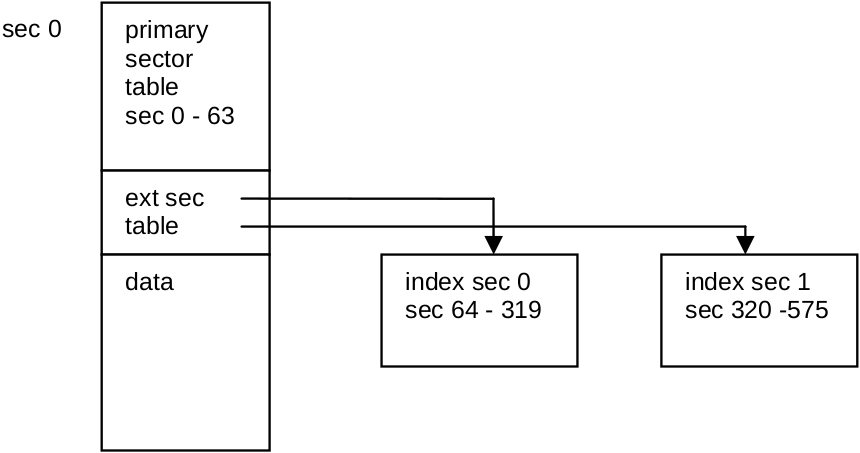
\includegraphics[width=\textwidth]{i/l}
	\caption{File header and extension sectors}
\end{figure}

The header contains some additional data, namely the length of the file (in bytes), its name, and
date and time of its creation. The size of the header is 352 bytes; the remaining 672 bytes of the
first sector are used for data. Hence, truly short files occupy a single sector only. The declaration
of the file header is contained in the definition of module FileDir. An abbreviated version
containing the fields relevant so far is:
\begin{verbatim}
FileHeader = RECORD
leng: INT;
ext: ARRAY 12 OF SectorPointer;
sec: ARRAY 64 OF SectorPointer
END
\end{verbatim}

We now turn our attention to the implementation of file access, and first present a system that
uses main storage for the file data instead of a disk and therefore avoids the problems introduced
by sector buffering. The key data structure in this connection is the Rider, represented as a
record.
\begin{verbatim}
Rider = RECORD
eof: BOOL; res, pos, adr: INT;
file: File
END
\end{verbatim}

A rider is initialised by a call Set(r, f, pos), which places the rider r on file f at position pos. From
this it is clear that the rider record must contain fields denoting the attached file and the rider's
position on it. We note that they are not exported. However, their values can be obtained by the
function procedures Pos(r) and Base(r). This allows a (hidden) representation most appropriate
for an efficient implementation of Read and Write without being unsafe.

Consider now the call Read(r, x); its task is to assign the value of the byte designated by the
rider's position to x and to advance the position to the next byte. Considering the structure by
which file data are represented, we easily obtain the following program, assuming that the
position is legal, i.e. non-negative and less than the file's length. a, b, c are local variables, HS is
the size of the header (in sector 0), SS is the sector size, typically a power of 2 in order to make
division efficient.
\begin{verbatim}
a := (r.pos + HS) DIV SS; b := (r.pos + HS) MOD SS;
IF a < 64 THEN c := r.file.sec[a]
ELSE c := r.file.ext[(a - 64) DIV 256].sec[(a - 64) MOD 256]
END ;
SYSTEM.GET(c + b, x) ; INC (r.pos)
\end{verbatim}

In order to gain efficiency, we use the low-level procedure GET that assigns the value at address
c+b to x. This program is reasonably short, but involves considerable address computations at
every access, and in particular at positions larger than 64 * SS. Fortunately, there exists an easy
remedy, namely that of caching the address of the current position. This explains the presence of
the field adr in the rider record. The resulting program is shown below; note that in order to avoid
the addition of HS, pos is defined to denote the genuine position, i.e. the abstract position
augmented by HS.
\begin{verbatim}
SYSTEM.GET(r.adr, x); INC(r.adr); INC(r.pos);
IF r.pos MOD SS = 0 THEN
m := r.pos DIV SS;
IF m < 64 THEN r.adr := r.file.sec[m]
ELSE r.adr := r.file.ext[(m - 64) DIV 256].sec[(m - 64) MOD 256]
END
END
\end{verbatim}

We emphasize that in all but one out of 1024 cases only three instructions and a single test are to
be executed. This improvement therefore is crucial to the efficiency of file access, and to that of
the entire Oberon. We now present the entire file module (for files on a random-access
store).
\begin{verbatim}
MODULE MFiles; (*NW 24.8.90 / 12.10.90 / 20.6.2013*)
IMPORT SYSTEM, Kernel, FileDir;
(*A file consists of a sequence of sectors. The first sector contains the header.
Part of the header is the sector table, an array of addresses to the sectors.
A file is referenced through riders each of which indicates a position.*)
CONST
HS = FileDir.HeaderSize;
SS = FileDir.SectorSize;
STS = FileDir.SecTabSize;
XS = FileDir.IndexSize;
TYPE File* = POINTER TO FileDesc;
Index = POINTER TO IndexRecord;
IndexRecord = RECORD sec: FileDir.IndexSector END ;
Rider* =
RECORD eof*: BOOL;
res*, pos, adr: INT;
file: File
END ;
FileDesc =
RECORD mark: INT;
name: FileDir.FileName;
len, date: INT;
ext: ARRAY FileDir.ExTabSize OF Index;
sec: FileDir.SectorTable
END ;
PROC Old*(name: ARRAY OF CHAR): File;
VAR head: INT;
namebuf: FileDir.FileName;
BEGIN
FileDir.Search(name, head); RETURN SYSTEM.VAL(File, head)
END Old;
PROC New*(name: ARRAY OF CHAR): File;
VAR f: File; head: INT;
BEGIN f := NIL; Kernel.AllocSector(0, head);
IF head $\neq$ 0 THEN
f := SYSTEM.VAL(File, head); f.mark := FileDir.HeaderMark;
f.len := HS; f.name := name;
f.date := Kernel.Clock(); f.sec[0] := head
END ;
RETURN f
END New;
PROC Register*(f: File);
BEGIN
IF (f $\neq$ NIL) & (f.name[0] > 0X) THEN FileDir.Insert(f.name, f.sec[0]) END ;
END Register;
PROC Length*(f: File): INT;
BEGIN RETURN f.len - HS
END Length;
PROC Date*(f: File): INT;
BEGIN RETURN f.date
END Date;
PROC Set*(VAR r: Rider; f: File; pos: LONGINT);
VAR m, n: INT;
BEGIN r.eof := FALSE; r.res := 0;
IF f $\neq$ NIL THEN
IF pos < 0 THEN r.pos := HS
ELSIF pos > f.len - HS THEN r.pos := f.len
ELSE r.pos := pos + HS
END ;
r.file := f; m := r.pos DIV SS; n := r.pos MOD SS;
IF m < STS THEN r.adr := f.sec[m] + n
ELSE r.adr := f.ext[(m-STS) DIV XS].sec[(m-STS) MOD XS] + n
END
END
END Set;
PROC ReadByte*(VAR r: Rider; VAR x: BYTE);
VAR m: INT;
BEGIN
IF r.pos < r.file.len THEN
SYSTEM.GET(r.adr, x); INC(r.adr); INC(r.pos);
IF r.adr MOD SS = 0 THEN
m := r.pos DIV SS;
IF m < STS THEN r.adr := r.file.sec[m]
ELSE r.adr := r.file.ext[(m-STS) DIV XS].sec[(m-STS) MOD XS]
END
END
ELSE x := 0; r.eof := TRUE
END
END ReadByte;
PROC WriteByte*(VAR r: Rider; x: BYTE);
VAR k, m, n, ix: INT;
BEGIN
IF r.pos < r.file.len THEN
m := r.pos DIV SS; INC(r.pos);
IF m < STS THEN r.adr := r.file.sec[m]
ELSE r.adr := r.file.ext[(m-STS) DIV XS].sec[(m-STS) MOD XS]
END
ELSE
IF r.adr MOD SS = 0 THEN
m := r.pos DIV SS;
IF m < STS THEN Kernel.AllocSector(0, r.adr); r.file.sec[m] := r.adr
ELSE n := (m - STS) DIV XS; k := (m - STS) MOD XS;
IF k = 0 THEN (*new index*)
Kernel.AllocSector(0, ix); r.file.ext[n] := SYSTEM.VAL(Index, ix)
END ;
Kernel.AllocSector(0, r.adr); r.file.ext[n].sec[k] := r.adr
END
END ;
INC(r.pos); r.file.len := r.pos
END ;
SYSTEM.PUT(r.adr, x); INC(r.adr)
END WriteByte;
PROC Pos*(VAR r: Rider): INT;
BEGIN RETURN r.pos - HS
END Pos;
PROC Base*(VAR r: Rider): File;
BEGIN RETURN r.file
END Base;
END MFiles.
\end{verbatim}

Allocation of a new sector occurs upon creating a file (Files.New), and when writing at the end of
a file after the current sector had been filled. Procedure AllocSector yields the address of the
allocated sector. It is determined by a search in the sector reservation table for a free sector. In
this table, every sector is represented by a single bit indicating whether or not the sector is
allocated. Although conceptually belonging to the FS, this table resides within module
Kernel.

Deallocation of a file's sectors could occur as soon as the file is no longer accessible, neither
through a variable of any loaded module nor from the file directory. However, this moment is
difficult to determine. Therefore, the method of garbage collection is used in Oberon for the
deallocation of file space. In consideration of the fact that file space is large and the collection of
unused sectors relatively time-consuming, we confine this process to system initialization. It is
represented by procedure FileDir.Init. At that time, the only referenced files are those registered
in the directory. Init therefore scans the entire directory and records the sectors referenced in
each file in the sector reservation table (see Sect. 7.4).

For applications where system startup and initialization is supposed to occur very infrequently,
such as for server systems, a procedure Files.Purge is provided. Its effect is to return the sectors
used by the specified file to the pool of free sectors. Evidently, the programmer then bears the
responsibility to guarantee that no references to the purged file continue to exist. This may be
possible in a closed server system, but files should not be purged under normal circumstances,
as a violation of said precondition will lead to unpredictable disaster.
The following procedures used for allocating, deallocating, and marking sectors in the sector
reservation table are defined in module Kernel:
\begin{verbatim}
PROC AllocSector(hint: INT; VAR sec: INT); (*used in WriteByte*)
PROC MarkSector(sec: INT); (*used in Init*)
PROC FreeSector(sec: INT); (*used in Purge*)
\end{verbatim}

\section{Implementation on a disk}
First we recall that the organization of files as sets of individually allocated blocks (sectors) is
inherently required by the allocation considerations of dynamically growing sequences. However,
if the storage medium is a tape, a disk, or a flash-RAM, there exists an additional reason for the
use of blocks. They constitute the subsequences to be individually buffered for transmission in
order to overcome the timing constraints imposed by the medium. If an adequate space utilization
is to be achieved, the blocks must not be too long. A typical size is 1, 2, or 4K bytes.
This necessity of buffering has a profound influence on the implementation of file access. The
complication arises because the abstraction of the sequence of individual bytes needs to be
maintained. The increase in complexity of file access is considerable, as can be seen by
comparing the program listings of the two respective implementations.

The first, obvious measure is to copy the file's sector table into primary store when a file is
"opened" through a call of New() or Old(). The record holding this copy is the file descriptor, and
the value f denoting the file points to this handle (instead of the actual header on disk). The
descriptor also contains the remaining information stored in the header, in particular the file's
length.

If a file is read (or written) in purely sequential manner, a single buffer is appropriate for the
transfer of data. For reading, the buffer is filled by reading a sector from the disk, and bytes are
picked up individually from the buffer. For writing, bytes are deposited individually, and the buffer
is written onto disk as a whole when full. The buffer is associated with the file, and a pointer to it
is contained in the descriptor.

However, we recall that several riders may be placed on a file and be moved independently. It
might be appealing to associate a buffer with each rider. But this proposal must quickly be
rejected when we realize that several riders may be active at neighbouring positions. If these
positions refer to the same sector, which is duplicated in the riders' distinct buffers, the buffers
may easily become inconsistent. Obviously, buffers must not be associated with riders, but with
the file itself. The descriptor therefore contains the head of a list of linked buffers. Each buffer is
identified by its position in the file. An invariant of the system is that no two buffers represent the
same sector.

Even with the presence of a single rider, the possibility of having several buffers associated with a
file can be advantageous, if a rider is frequently repositioned. It becomes a question of strategy
and heuristics when to allocate a new buffer. In the Oberon, we have adopted the
following solution:
\begin{enumerate}
	\item The first buffer is created when the file is opened (New, Old).
	\item Additional buffers may be allocated when a rider is placed (or repositioned) on the file.
	\item At most four buffers are connected to the same file.
	\item Purely sequential movements of riders do not cause allocation of buffers.
	\item Separate buffers are generated when extensions of the file's sector table need be accessed
(rider position > 64K). Each buffers the 256 sector addresses of the respective index sector.
\end{enumerate}

The outlined scheme requires and is based upon the following data structures and types:
\begin{verbatim}
File =
Buffer =
Index =

POINTER TO FileDesc;
POINTER TO BufferRecord;
POINTER TO IndexRecord;

FileDesc = RECORD next: File;
aleng, bleng: INT;
(*file length*)
nofbufs: INT; (*no. of buffers allocated*)
modH, registered: BOOL; (*header has been modified*)
firstbuf: Buffer:
(*head of buffer chain*)
sechint: DiskAdr;
(*sector hint*)
name: FileDir.FileName;
date: INT;
ext: ARRAY FileDir.ExTabSize OF Index;
sec: ARRAY 64 OF DiskAdr
END;
BufferRecord = RECORD apos, lim: INT; (*lim = no. of bytes*)
mod: BOOL;
(*buffer has been modified*)
next: Buffer;
(*buffer chain*)
data: FileDir.DataSector
END;
IndexRecord = RECORD adr: DiskAdr;
mod: BOOL;
(*index record has been modified*)
sec: FileDir.IndexSector
END;
Rider =

RECORD eof: BOOL;
res: INT;
file: File;
apos, bpos: INT;
buf: Buffer
END ;

(*end of file reached*)
(*no. of unread bytes*)
(*position*)
(*hint: likely buffer*)
\end{verbatim}

In order to increase efficiency of access, riders have been provided with a field containing the
address of the element of the rider's position. From the conditions stated above for the allocation
of buffers, it is evident that the value of this field can be a hint only. This implies that there can be
no reliance on its information. Whenever it is used, its validity has to be checked. The check
consists in a comparison of the riders' position r.apos with the hinted buffer's actual position
r.buf.apos. If they differ, a buffer with the desired position must be searched and, if not present,
allocated. The advantage of the hint lies in the fact that the hint is correct with a very high
probability. The check is included in procedures Read, ReadByte, Write, and WriteByte.
Some fields of the record types require additional explanations:

\begin{enumerate}
	\item The length is stored in a "preprocessed" form, namely by the two integers aleng and bleng
such that aleng is a sector number and
\begin{verbatim}
length = (aleng * SS) + bleng - HS
aleng = (length + HS) DIV SS
bleng = (length + HS) MOD SS
\end{verbatim}
The same holds for the form of the position in riders (apos, bpos).
	\item The field nofbufs indicates the number of buffers in the list headed by firstbuf:
\begin{verbatim}
1 <= nofbufs <= Maxbufs.
\end{verbatim}
	\item Whenever data are written into a buffer, the file becomes inconsistent, i.e. the data on the disk
are outdated. The file is updated, i.e. the buffer is copied into the corresponding disk sector,
whenever the buffer is reallocated, e.g. during sequential writing after the buffer is full and is
"advanced". During sequential reading, a buffer is also advanced and reused, but needs not be
copied onto disk, because it is still consistent. Whether a buffer is consistent or not is indicated by
its state variable mod (modified). Similarly, the field modH in the file descriptor indicates whether
or not the header had been modified.
	\item The field sechint records the number of the last sector allocated to the file and serves as a hint
to the kernel's allocation procedure, which allocates a next sector with an address larger than the
hint. This is a measure to gain speed in sequential scans.
	\item The buffer's position is specified by its field apos. Used as index in the file header's sector
table, it yields the sector corresponding to the current buffer contents. The field lim specifies the
number of bytes s stored in the buffer. Reading cannot proceed beyond this limiting index; writing
beyond it implies an increase in the file's length. All buffers except the one for the last sector are
filled and specify lim = SS.
	\item The hidden rider field buf is merely a hint to speed up localization of the concerned buffer. A
hint is likely, but not guaranteed to be correct. Its validity must be checked before use. The buffer
hint is invalidated when a buffer is reallocated and/or a rider is repositioned.
The structure of riders remains practically the same as for files using main store. The hidden field
adr is merely replaced by a pointer to the buffer covering the rider's position. A configuration of a
file f with two riders is shown in Fig \ref{fig:file}.
	\begin{figure}
		\flushright
		\label{fig:file}
		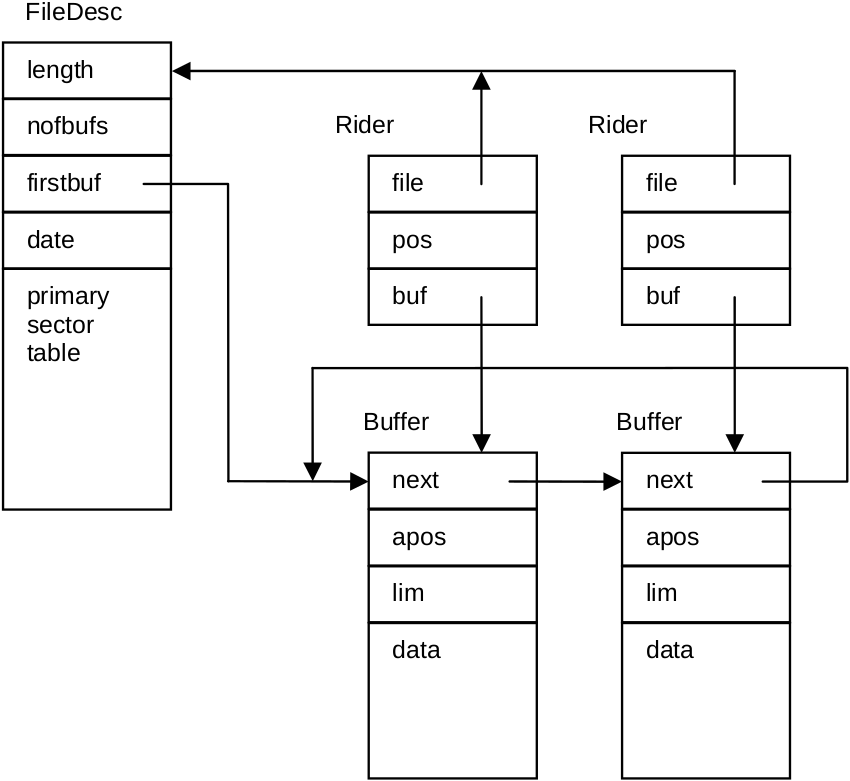
\includegraphics[width=.9\textwidth]{i/m}
		\caption{File $f$ with two riders and two buffers}
	\end{figure}
\end{enumerate}

Some comments concerning module Files follow.
\begin{enumerate}
	\item After the writing of a file has been completed, its name is usually registered in the directory.
Register invokes procedure Unbuffer. It inspects the associated buffers and copies those onto
disk which had been modified. During this process, new index sectors may have to be transferred
as well. If a file is to remain anonymous and local to a module or command, i.e. is not to be
registered, but merely to be read, the release of buffers must be specified by an explicit call to
Close (meaning "close buffers"), which also invokes Unbuffer.
	\item Procedure Old (and for reasons of consistency also New) deviates from the general Oberon
programming rule that an object be allocated by the calling (instead of the called) module. This
rule would suggest the statements
\[ New(f); Files.Open(f, name) \] instead of \[ f := Files.Old(name). \] The justification for the rule is that any extension of the type of f
could be allocated, providing for more flexibility. And the reason for our deviation in the case of
files is that, upon closer inspection, not a new file, but only a new descriptor is to be allocated.
The distinction becomes evident when we consider that several statements
$f := Files.Old(name)$ with different $f$ and identical name may occur, probably in different modules. In this case, it is
necessary that the same descriptor is referenced by the delivered pointers in order to avoid file
inconsistency. Each (opened) file must have exactly one descriptor. When a file is opened, the
first action is therefore to inspect whether a descriptor of this file already exists. For this purpose,
all descriptors are linked together in a list anchored by the global variable root and linked by the
descriptor field next. This measure may seem to solve the problem of avoiding inconsistencies
smoothly. However, there exists a pitfall that is easily overlooked: All opened files would
permanently remain accessible via root, and the garbage collector could never remove a file
descriptor nor its associated buffers. This would be unacceptable. In order to hide this list from
the garbage collector, it is represented by integers (addresses) instead of pointers.
	\item Sector pointers are represented by sector numbers of type $INT$. Actually, we use the
numbers multiplied by 29. This implies that any single-bit error leads to a number which is not a
multiple of 29, and hence can easily be detected. Thereby the crucial sector addresses are
software parity checked and are safe (against single-bit errors) even on computers without
hardware parity check. The check is performed by procedures $Kernel.GetSector$ and $Kernel.PutSector$.
\end{enumerate}

\section{The file directory}
A directory is a set of pairs, each pair consisting of a name (key) and an object (here: file). It
serves to retrieve objects by their name. If efficiency matters, the directory is organized as an
ordered set, ordered according to the keys. The most frequently used structures for ordered sets
are trees and hash tables. The latter have disadvantages when the size of the set is unknown,
particularly when its order of magnitude is unknown, and when deletions occur. The Oberon
system therefore uses a tree structure for its file directory, more specifically a B-tree, which was
developed especially for cases where not individual pairs, but only sets of pairs as a whole
(placed on a disk sector) can be accessed.

For a thorough study of B-trees we refer the reader to the literature [1, 2]. Here it must suffice to
specify the B-tree's principal characteristics:
\begin{enumerate}
	\item In a B-tree of order $N$, each node (called page) contains $m$ elements (pairs), where $N \leq m \leq
2N$, except the root, where $0 \leq m \leq 2N$.
	\item A page with $m$ elements has either $0$ descendants, in which case it is called a leaf page, or $m + 1$ descendants.
	\item All leaf pages are on the same (bottom) level.
\end{enumerate}
From 3, it follows that the B-tree is a balanced tree. Its height, and with it the longest path's
length, has an upper bound of, roughly, $2 * \log{k}$, where $k$ is the number of elements and the
logarithm is taken to the base $N$ and rounded up to the next larger integer. Its minimal height is
$\log{k}$ taken to the base $2N$.

On each page, space must be available for $2N$ elements and for $2N + 1$ references to
descendants. Hence, $N$ is immediately determined by the size of a page and the size of elements.
In the case of Oberon, names are limited to 32 characters (bytes), and the object is a
reference to the associated file (4 bytes). Each descendant pointer takes 4 bytes, and the page
size is given by the sector size (1024) minus the number of bytes needed to store $m$ (2 bytes).
Hence
\begin{verbatim}
  N = ((1024 - 2 - 4) DIV (32 + 4 + 4)) DIV 2 = 12
\end{verbatim}
A B-tree of height h and order 12 may contain the following minimal and maximal number of
elements:
\begin{table}
	\centering
	\begin{tabular}{c r r}
		height & minimum & maximum \\
		1      &       0 &      24 \\
		2      &      25 &     624 \\
		3      &     625 &   15624 \\
		4      &   15625 &  390624 \\
	\end{tabular}
\end{table}

It follows that the height of the B-tree will never be larger than 4, if the disk has a capacity of less
than about 400 Mbyte, and assuming that each file occupies a single 1K sector. It is rarely larger
than 3 in practice.

The definition of module FileDir shows the available directory operations. Apart from the
procedures Search, Insert, Delete, and Enumerate, it contains some data definitions, and it
should be considered as the non-public part of the FS's interface.
\begin{verbatim}
DEFINITION FileDir;
IMPORT SYSTEM, Kernel;
CONST
FnLength = 32;
(*max length of file name*)
SecTabSize = 64; (*no. of entries in primary table*)
ExTabSize = 12;
SectorSize = 1024;
IndexSize = SectorSize DIV 4;
(*no. of entries in index sector*)
HeaderSize = 352;
DirRootAdr = 29;
DirPgSize = 24;
(*max no. of elements on page*)
TYPE DiskAdr = INT;
FileName = ARRAY FnLength OF CHAR;
SectorTable = ARRAY SecTabSize OF DiskAsr;
ExtensionTable = ARRAY ExTabSize OF DiskAdr;
EntryHandler = PROC (name: FileName; sec: DiskAdr; VAR continue: BOOL);
FileHeader = RECORD (*first page of each file on disk*)
mark: INT;
name: FileName;
aleng, bleng, date: INT;
ext: ExtensionTable;
sec: SectorTable
END ;
IndexSector = RECORD (Kernel.Sector)
x: ARRAY IndexSize OF LONGINT;
END ;
DataSector = ARRAY SectorSize OF BYTE;
DirEntry = RECORD
name: FileName;
adr, p: DiskAdr
END ;
DirPage = RECORD
mark: INT;
m: INT; (*no. of elements on page*)
p0: DiskAdr;
e: ARRAY DirPgSize OF DirEntry;
END ;
PROC Search(name: FileName; VAR fad: DiskAdr);
PROC Insert(name: FileName; fad: DiskAdr);
PROC Delete(name: FileName; VAR fad: DiskAdr);
PROC Enumerate(prefix: ARRAY OF CHAR; proc: EntryHandler);
END FileDir.
\end{verbatim}

Procedures Search, Insert, and Delete represent the typical operations performed on a directory.
Efficiency of the first operation is of primary importance. But the B-tree structure also guarantees
efficient insertion and deletion, although the code for these operations is complex. Procedure
Enumerate is used to obtain excerpts of the directory. The programmer must guarantee that no
directory changes are performed by the parametric procedure of Enumerate.

As in the presentation of module Files, we first discuss a version that uses main storage rather
than a disk for the directory. This allows us to concentrate on the algorithms for handling the
directory, leaving out the additional complications due to the necessity to read pages (sectors)
into main store for selective updating and of restoring them onto disk. In particular, we point out
the definitions of the data types for B-tree nodes, called DirPage, and elements, called DirEntry.
The component E.p of an entry E points to the page in which all elements (with index k) have
keys E.p.e[k].name > E.name. The pointer p.p0 points to a page in which all elements have keys
p.p0.e[k].name < p.e[0].name. We can visualize these conditions by Fig. \ref{fig:b-tree}, where names have
been replaced by integers as keys.
\begin{figure}
	\label{fig:b-tree}
	\centering
	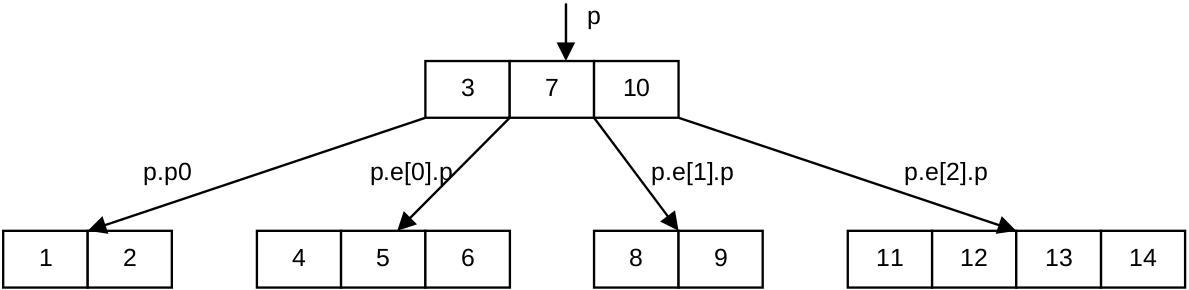
\includegraphics[width=\textwidth]{i/n}
	\caption{Example of a B-tree of order 2}
\end{figure}

Procedure $Search$ starts by inspecting the root page. It performs a binary search among its
elements, according to the following algorithm. Let $e[0 \dots m-1]$ be the ordered keys and $x$ the
search argument.
\begin{verbatim}
L := 0; R := m;
WHILE L < R DO
i := (L+R) DIV 2;
IF x <= e[i] THEN R := i ELSE L := i + 1 END
END;
IF (R < m) & (x = e[R]) THEN found END
\end{verbatim}

The invariant is
\[ e[L-1] < x \leq e[R] \]
If the desired element is not found, the search continues on the appropriate descendant page, if
there is one. Otherwise the element is not contained in the tree.

Procedures insert and delete use the same algorithm for searching an element within a page.
However, they use recursion instead of iteration to proceed along the search path of pages. We
recall that the depth of recursion is at most four. The reason for the use of recursion is that it
facilitates the formulation of structural changes, which are performed during the "unwinding" of
recursion, i.e. on the return path. First, the insertion point (respectively the position of the element
to be deleted) is searched, and then the element is inserted (deleted).

Upon insertion, the number of elements on the insertion page may become larger than $2N$,
violating B-tree condition 1. This situation is called page overflow. The invariant must be
reestablished immediately. It could be achieved by moving one element from either end of the
array e onto a neighbouring page. However, we choose not to do this, and instead to split the
overflowing page into two pages immediately. The process of a page split is visualized by Fig \ref{fig:page-split},
in which we distinguish between three cases, namely $R < N$, $R = N$, and $R > N$, where $R$ marks
the insertion point. $a$ denotes the overflowing, $b$ the new page, and $u$ the inserted element.
The $2N + 1$ elements ($2N$ from the full page $a$, plus the one element $u$ to be inserted) are equally
distributed onto pages $a$ and $b$. One element $v$ is pushed up in the tree. It must be inserted in the
ancestor page of $a$. Since that page obtains an additional descendant, it must also obtain an
additional element in order to maintain B-tree rule 2.

A page split may thus propagate, because the insertion of element $v$ in the ancestor page may
require a split once again. If the root page is full, it is split too, and the emerging element $v$ is
inserted in a new root page containing a single element. This is the only way in which the height
of a B-tree can increase.

\begin{figure}
	\label{fig:page-split}
	\centering
	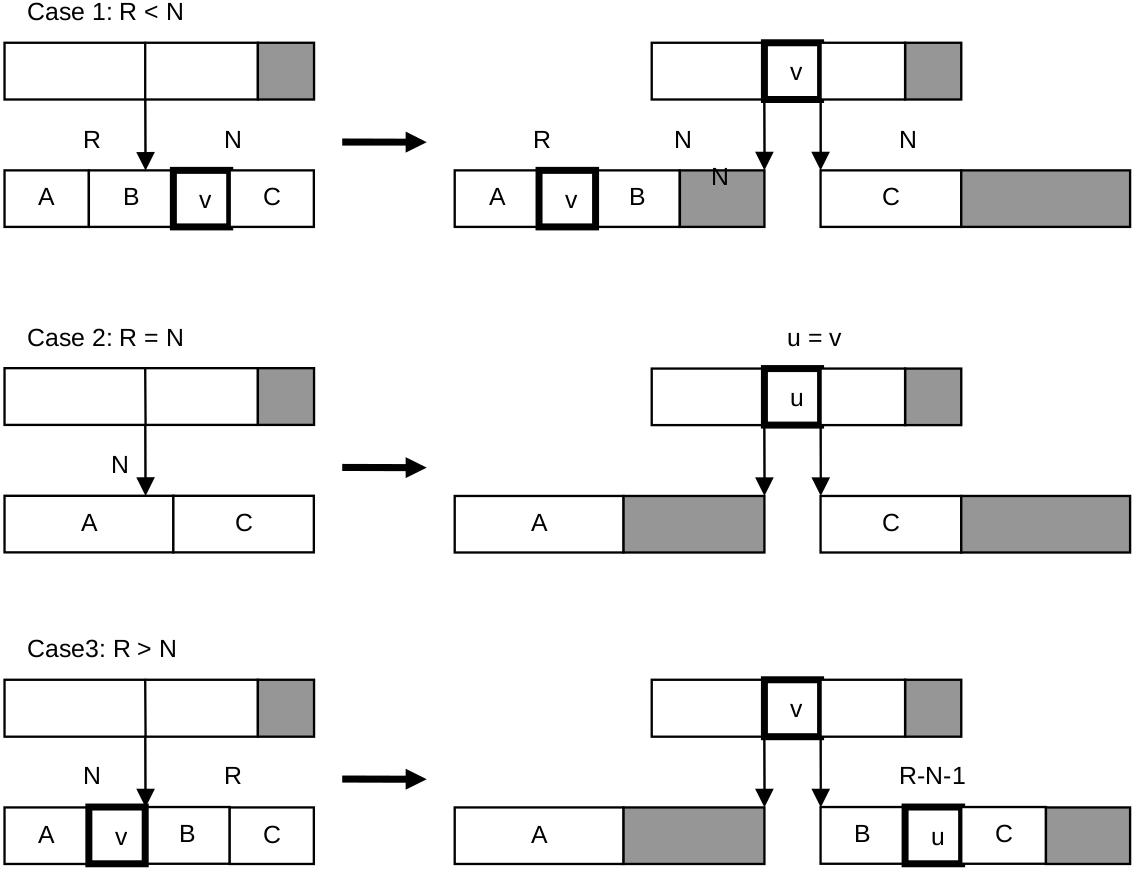
\includegraphics[width=.95\textwidth]{i/o}
	\caption{Page split when inserting element $u$}
\end{figure}
When an element is to be deleted, it cannot simply be removed, if it resides on an internal page.
In this case, it is first replaced by another element, namely one of the two neighbouring elements
on a leaf page, i.e. the next smaller (or next larger) element, which is always on a leaf page. In
the presented solution, the replacing element is the largest on the left subtree (see procedure
del). Hence, the actual deletion always occurs on a leaf page.

Upon deletion, the number of elements in a page may become less than $N$, violating invariant 1.
This event is called page underflow. Since restructuring the tree is a relatively complicated
operation, we first try to reestablish the invariant by borrowing an element from a neighbouring
page. In fact, it is reasonable to borrow several elements, and thereby to decrease the likelihood
of an underflow on the same page upon further deletions. The number of elements that could be
taken from the neighbouring page $b$ is $b.m - N$. Hence we will borrow
\begin{verbatim}
  k = (b.m - N + 1) DIV 2
\end{verbatim}
elements. The process of page balancing then distributes the elements of the underflowing and
its neighbouring page equally to both pages (see procedure underflow).
However, if (and only if) the neighbouring page has no elements to spare, the two pages can and
must be united. This action, called page merge, places the $N-1$ elements from the underflowing
page, the $N$ elements from the neighbouring page, plus one element from the ancestor page onto
a single page of size $2N$. One element must be taken from the ancestor page, because that page
loses one descendant and invariant rule 2 must be maintained. The events of page balancing and
merging are illustrated in Fig \ref{fig:page-merge}. $a$ is the underflowing page, $b$ its neighbouring page, and $c$ their
ancestor; $s$ is the position in the ancestor page of (the pointer to the) underflowing page $a$. Two
cases are distinguished, namely whether the underflowing page is the rightmost element ($s =
c.m$) or not (see procedure underflow).

\begin{figure}
	\label{fig:page-merge}
	\centering
	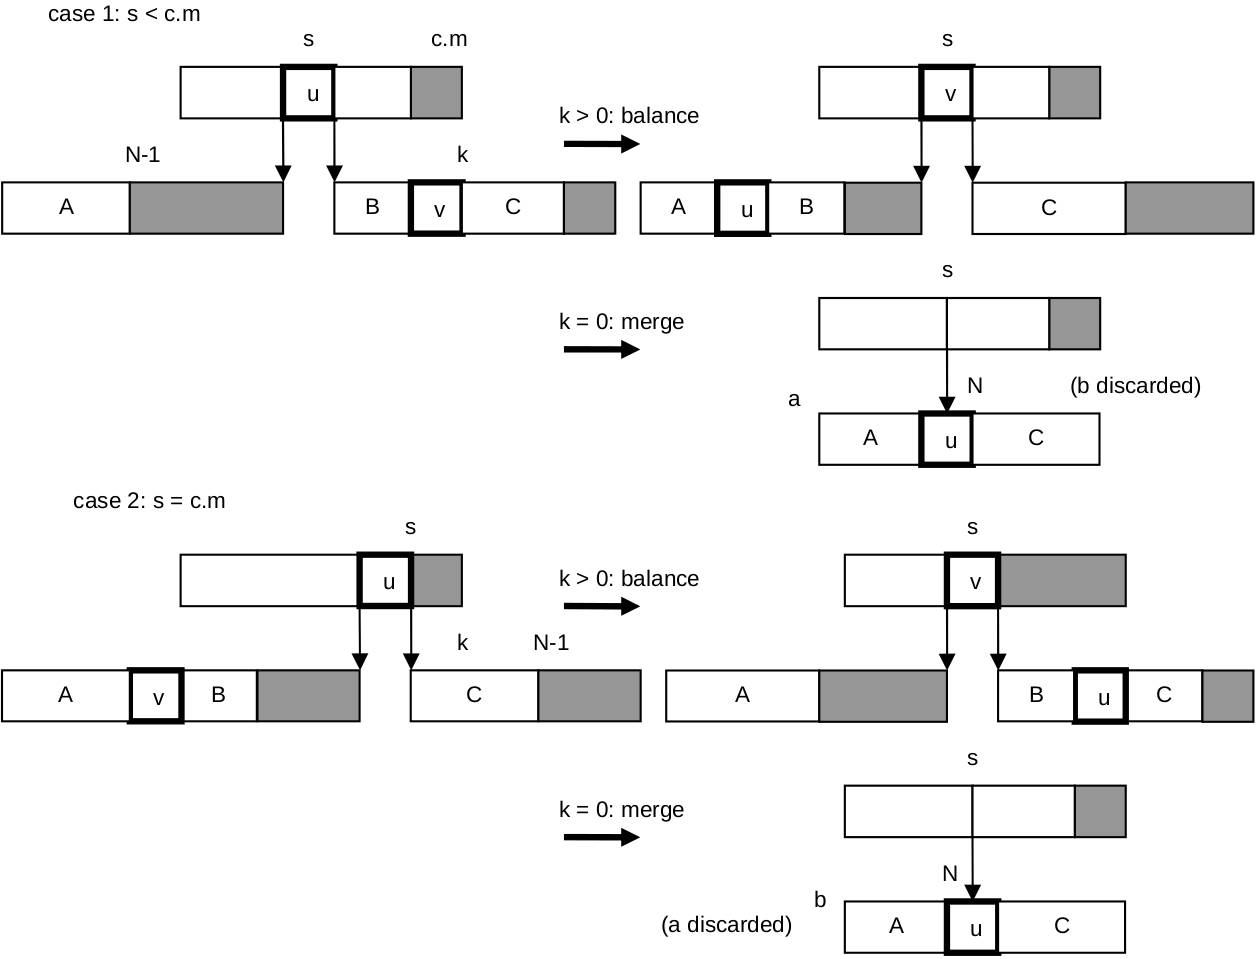
\includegraphics[width=.95\textwidth]{i/p}
	\caption{Page balancing and merging when deleting element}
\end{figure}
Similarly to the splitting process, merging may propagate, because the removal of an element
from the ancestor page may again cause an underflow, and perhaps a merge. The root page
underflows only if its last element is removed. This is the only way in which the B-tree's height
can decrease.
\begin{verbatim}
MODULE BTree;
IMPORT Texts, Oberon;
CONST N = 3;
TYPE Page = POINTER TO PageRec;
Entry = RECORD
key, data: INT;
p: Page
END ;
PageRec = RECORD
m: INT; (*no. of entries on page*)
p0: Page;
e: ARRAY 2*N OF Entry
END ;
VAR root: Page; W: Texts.Writer;
PROC search(x: INT; VAR p: Page; VAR k: INT);
VAR i, L, R: INT; found: BOOL; a: Page;
BEGIN a := root; found := FALSE;
WHILE (a $\neq$ NIL) & ~found DO
L := 0; R := a.m; (*binary search*)
WHILE L < R DO
i := (L+R) DIV 2;
IF x <= a.e[i].key THEN R := i ELSE L := i+1 END
END ;
IF (R < a.m) & (a.e[R].key = x) THEN found := TRUE
ELSIF R = 0 THEN a := a.p0 ELSE a := a.e[R-1].p
END
END ;
p := a; k := R
END search;
PROC insert(x: INT; a: Page; VAR h: BOOL; VAR v: Entry);
(*a $\neq$ NIL. Search key x in B-tree with root a; if found, increment counter.
Otherwise insert new item with key x. If an entry is to be passed up,
assign it to v. h := "tree has become higher"*)
VAR i, L, R: INT;
b: Page; u: Entry;
BEGIN (*a $\neq$ NIL & ~h*)
L := 0; R := a.m; (*binary search*)
WHILE L < R DO
i := (L+R) DIV 2;
IF x <= a.e[i].key THEN R := i ELSE L := i+1 END
END ;
IF (R < a.m) & (a.e[R].key = x) THEN (*found*) INC(a.e[R].data)
ELSE (*item not on this page*)
IF R = 0 THEN b := a.p0 ELSE b := a.e[R-1].p END ;
IF b = NIL THEN (*not in tree, insert*)
u.p := NIL; h := TRUE; u.key := x
ELSE insert(x, b, h, u)
END ;
IF h THEN (*insert u to the left of a.e[R]*)
IF a.m < 2*N THEN
h := FALSE; i := a.m;
WHILE i > R DO DEC(i); a.e[i+1] := a.e[i] END ;
a.e[R] := u; INC(a.m)
ELSE NEW(b); (*overflow; split a into a,b and assign the middle entry to v*)
IF R < N THEN (*insert in left page a*)
i := N-1; v := a.e[i];
WHILE i > R DO DEC(i); a.e[i+1] := a.e[i] END ;
a.e[R] := u; i := 0;
WHILE i < N DO b.e[i] := a.e[i+N]; INC(i) END
ELSE (*insert in right page b*)
DEC(R, N); i := 0;
IF R = 0 THEN v := u
ELSE v := a.e[N];
WHILE i < R-1 DO b.e[i] := a.e[i+N+1]; INC(i) END ;
b.e[i] := u; INC(i)
END ;
WHILE i < N DO b.e[i] := a.e[i+N]; INC(i) END
END ;
a.m := N; b.m := N; b.p0 := v.p; v.p := b
END
END
END
END insert;
PROC underflow(c, a: Page; s: INT; VAR h: BOOL);
(*a = underflowing page, c = ancestor page,
s = index of deleted entry in c*)
VAR b: Page;
i, k: INT;
BEGIN (*h & (a.m = N-1) & (c.e[s-1].p = a) *)
IF s < c.m THEN (*b := page to the right of a*)
b := c.e[s].p; k := (b.m-N+1) DIV 2; (*k = nof items available on page b*)
a.e[N-1] := c.e[s]; a.e[N-1].p := b.p0;
IF k > 0 THEN (*balance by moving k-1 items from b to a*) i := 0;
WHILE i < k-1 DO a.e[i+N] := b.e[i]; INC(i) END ;
c.e[s] := b.e[k-1]; b.p0 := c.e[s].p;
c.e[s].p := b; DEC(b.m, k); i := 0;
WHILE i < b.m DO b.e[i] := b.e[i+k]; INC(i) END ;
a.m := N-1+k; h := FALSE
ELSE (*merge pages a and b, discard b*) i := 0;
WHILE i < N DO a.e[i+N] := b.e[i]; INC(i) END ;
i := s; DEC(c.m);
WHILE i < c.m DO c.e[i] := c.e[i+1]; INC(i) END ;
a.m := 2*N; h := c.m < N
END
ELSE (*b := page to the left of a*) DEC(s);
IF s = 0 THEN b := c.p0 ELSE b := c.e[s-1].p END ;
k := (b.m-N+1) DIV 2; (*k = nof items available on page b*)
IF k > 0 THEN i := N-1;
WHILE i > 0 DO DEC(i); a.e[i+k] := a.e[i] END ;
i := k-1; a.e[i] := c.e[s]; a.e[i].p := a.p0;
(*move k-1 items from b to a, one to c*) DEC(b.m, k);
WHILE i > 0 DO DEC(i); a.e[i] := b.e[i+b.m+1] END ;
c.e[s] := b.e[b.m]; a.p0 := c.e[s].p;
c.e[s].p := a; a.m := N-1+k; h := FALSE
ELSE (*merge pages a and b, discard a*)
c.e[s].p := a.p0; b.e[N] := c.e[s]; i := 0;
WHILE i < N-1 DO b.e[i+N+1] := a.e[i]; INC(i) END ;
b.m := 2*N; DEC(c.m); h := c.m < N
END
END
END underflow;
PROC delete(x: INT; a: Page; VAR h: BOOL);
(*search and delete key x in B-tree a; if a page underflow arises,
balance with adjacent page or merge; h := "page a is undersize"*)
VAR i, L, R: INT; q: Page;
PROC del(p: Page; VAR h: BOOL);
VAR k: INT; q: Page; (*global a, R*)
BEGIN k := p.m-1; q := p.e[k].p;
IF q $\neq$ NIL THEN del(q, h);
IF h THEN underflow(p, q, p.m, h) END
ELSE p.e[k].p := a.e[R].p; a.e[R] := p.e[k];
DEC(p.m); h := p.m < N
END
END del;
BEGIN (*a $\neq$ NIL*)
L := 0; R := a.m; (*binary search*)
WHILE L < R DO
i := (L+R) DIV 2;
IF x <= a.e[i].key THEN R := i ELSE L := i+1 END
END ;
IF R = 0 THEN q := a.p0 ELSE q := a.e[R-1].p END ;
IF (R < a.m) & (a.e[R].key = x) THEN (*found*)
IF q = NIL THEN (*a is leaf page*)
DEC(a.m); h := a.m < N; i := R;
WHILE i < a.m DO a.e[i] := a.e[i+1]; INC(i) END
ELSE del(q, h);
IF h THEN underflow(a, q, R, h) END
END
ELSE delete(x, q, h);
IF h THEN underflow(a, q, R, h) END
END
END delete;
PROC Search*(key: INT; VAR data: INT);
BEGIN search(key, root, data)
END Search;
PROC Insert*(key: INT; VAR data: INT);
VAR h: BOOL; u: Entry; q: Page;
BEGIN h := FALSE; u.data := data; insert(key, root, h, u);
IF h THEN (*insert new base page*)
q := root; NEW(root);
root.m := 1; root.p0 := q; root.e[0] := u
END
END Insert;
PROC Delete*(key: INT);
VAR h: BOOL;
BEGIN h := FALSE; delete(key, root, h);
IF h THEN (*base page size underflow*)
IF root.m = 0 THEN root := root.p0 END
END
END Delete;
BEGIN NEW(root); root.m := 0
END BTree.
\end{verbatim}

The B-tree is also a highly appropriate structure for enumerating its elements, because during the
traversal of the tree each page is visited exactly once, and hence needs to be read (from disk)
exactly once too. The traversal is programmed by the procedure Enumerate and uses recursion.
It calls the parametric procedure proc for each element of the tree. The type of proc specifies as
parameters the name and the (address of) the enumerated element. The third parameter
continue is a Boolean VAR-parameter. If the procedure sets it to FALSE, the process of
enumeration will be aborted.

Enumerate is used for obtaining listings of the names of registered files. For this purpose, the
actual procedure substituted for proc merely enters the given name in a text and ignores the
address (sector number) of the file, unless it requires special file information such as the file's
size or creation date.

The set of visited elements can be restricted by specifying a string which is to be a prefix to all
enumerated names. The least name with the specified prefix is directly searched and is the name
(key) of the first element enumerated. The process then proceeds up to the first element whose
name does not have the given prefix. Thereby, the process of obtaining all elements whose key
has a given prefix avoids traversal of the whole tree, resulting in a significant speedup. If the
prefix is the empty string, the entire tree is traversed.

The principle behind procedure Enumerate is shown by the following sketch, where we abstract
from the B-tree structure and omit consideration of prefixes:
\begin{verbatim}
PROC Enumerate(
proc: PROC (name: FileName; adr: INT; VAR continue: BOOL));
VAR continue: BOOL; this: DirEntry;
BEGIN continue := TRUE; this := FirstElement;
WHILE continue & (this $\neq$ NIL) DO
proc(this.name, this.adr, continue); this := NextEntry(this)
END
END Enumerate
\end{verbatim}
From this sketch we may conclude that during the process of traversal the tree structure must not
change, because the function NextEntry quite evidently relies on the structural information stored
in the elements of structure itself. Hence, the actions of the parametric procedure must not affect
the tree structure. Enumeration must not be used, for example, to delete a given set of files. In
order to prevent the misuse of the indispensible facility of element enumeration, the interface of
FileDir is not available to users in general.

The handling of the directory stored on disk follows exactly the same algorithms. The accessed
pages are fetched from the disk as a whole (each page fits onto a single disk sector) and stored
in buffers of type DirPage, from where individual elements can be accessed. In principle, these
buffers can be local to procedures insert and delete. A single buffer is allocated globally, namely
the one used by procedure Search. The reason for this exception is not only that iterative
searching requires one buffer only, but because procedure Files.Old and in turn Search may be
called when the processor is in the supervisor mode and hence uses the system- (instead of the
user-) stack, which is small and would not accommodate sector buffers.

Naturally, an updated page needs to be stored back onto disk. Omission of sector restoration is a
programming error that is very hard to diagnose, because some parts of the program are
executed very rarely, and hence the error may look sporadic and mistakenly be attributed to
malfunctioning hardware.

Oberon's file directory represents a single, ordered set of name-file pairs. It is therefore also
called a flat directory. Its internal tree structure is not visible to the outside. In contrast, some file
systems use a directory with a visible tree structure, notably UNIX. In a search, the name (key)
guides the search path; the name itself displays structure, in fact, it is a sequence of names
(usually separated by slashes or periods). The first name is then searched in the root directory,
whose descendants are not files but subdirectories. The process is repeated, until the last name
in the sequence has been used (and hopefully denotes a file).

Since the search path length in a tree increases with the logarithm of the number of elements,
any subdivision of the tree inherently decreases performance since log(m + n) < log(m) + log (n)
for any m, n > 1. It is justified only if there exist sets of elements with common properties. If these
property values are stored once, namely in the subdirectory referencing all elements with
common property values, instead of in every element, not only a gain in storage economy results,
but possibly also in accesses which depend on those properties. The common properties are
typically an owner's name, a password, and access rights (read or write protection), properties
that primarily have significance in a multi-user environment. Since Oberon was conceived
explicitly as a single-user system, there is little need for such facilities, and hence a flat directory
offers the best performance with a simple implementation.

Every directory operation starts with an access to the root page. An obvious measure for
improving efficiency is to store the root page "permanently" in main store. We have chosen not to
do this for four reasons:
\begin{enumerate}
	\item If the hardware fails, or if the computer is switched off before the root page is copied to disk,
the file directory will be inconsistent with severe consequences.
	\item The root page has to be treated differently from other pages, making the program more
complex.
	\item Directory accesses do not dominate the computing process; hence, any improvement would
hardly be noticeable in overall system performance. The payoff for the added complexity would
be small.
	\item Procedure $Init$ is called upon system initialization in order to construct the sector reservation
table. Therefore, this procedure (and the module) must be allowed to refer to the structure of a
file's sector table(s), which is achieved by placing its definitions into the module $FileDir$ (instead of
$Files$). Unlike $Enumerate$, $Init$ traverses the entire B-tree. The sector numbers of files delivered by
$TraverseDir$ are entered into a buffer. When full, the entries are sorted, whereafter each file's
head sector is read and the sectors indicated in its sector table are marked as reserved. The
sorting speeds up the reading of the header sectors considerably. Nevertheless, the initialization
of the sector reservation table clearly dominates the start-up time of the computer. For a file
system with 10,000 files it takes in the order of 15s to record all files.
\end{enumerate}

\section{The toolbox of file utilities}
We conclude this chapter with a presentation of the commands which constitute the toolbox for
file handling. These commands are contained in the tool module $System$, and they serve to copy,
rename, and delete files, and to obtain excerpts of the file directory.
Procedures $CopyFiles$, $RenameFiles$, and $DeleteFiles$ all follow the same pattern. The parameter
text is scanned for file names, and for each operation a corresponding procedure is called. If the
parameter text contains an arrow, it is interpreted as a pointer to the most recent text selection
which indicates the file name. In the cases of $CopyFiles$ and $RenameFiles$ which require two
names for a single action, the names are separated by "$\Rightarrow$" indicating the direction of the copy or
rename actions.

Procedure $Directory$ serves to obtain excerpts of the file directory. It makes use of procedure
$FileDir.Enumerate$. The parametric procedure $List$ tests whether or not the delivered name
matches the pattern specified by the parameter of the directory command. If it matches, the name
is listed in the text of the viewer opened in the system track. Since the pattern may contain one or
several asterisks (wild cards), the test consists of a sequence of searches of the pattern parts
(separated by the asterisks) in the file name. In order to reduce the number of calls of $List$,
$Enumerate$ is called with the first part of the pattern as parameter prefix. Enumeration then starts
with the least name having the specified prefix, and terminates as soon as all names with this
prefix have been scanned.

If the specified pattern is followed by an option directive "!", then not only file names are listed, but
also the listed files' creation date and length. This requires that not only the directory sectors on
the disk are traversed, but that additionally for each listed file its header sector must be read. The
two procedures use the global variables $pat$ and $diroption$.

\section*{References}
\begin{enumerate}
	\item R. Bayer and E. M. McCreight. Organization and maintenance of large ordered indexes. Acta Informatica, 1, 3, (1972), 173-189.

	\item D. Comer. The ubiquitous B-tree. ACM Comp Surveys, 11, 2, (June 1979), 121-137.
\end{enumerate}
